\begin{appendices}
\FloatBarrier
\begin{figure}[h]
\section*{Bilag 1}\label{bilag1}
\centering
\makebox[\textwidth]{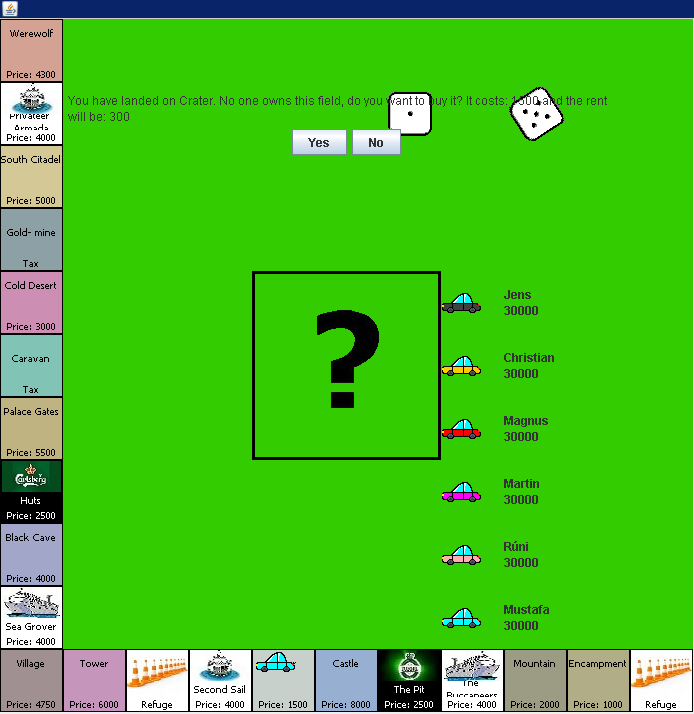
\includegraphics[width=0.8\paperwidth]{bilag01}}
\caption{\emph{Bilag 1}: Spilleren tilbydes at købe et felt.}
\end{figure}
\FloatBarrier
\begin{figure}[h]
\section*{Bilag 2}\label{bilag2}
\centering
\makebox[\textwidth]{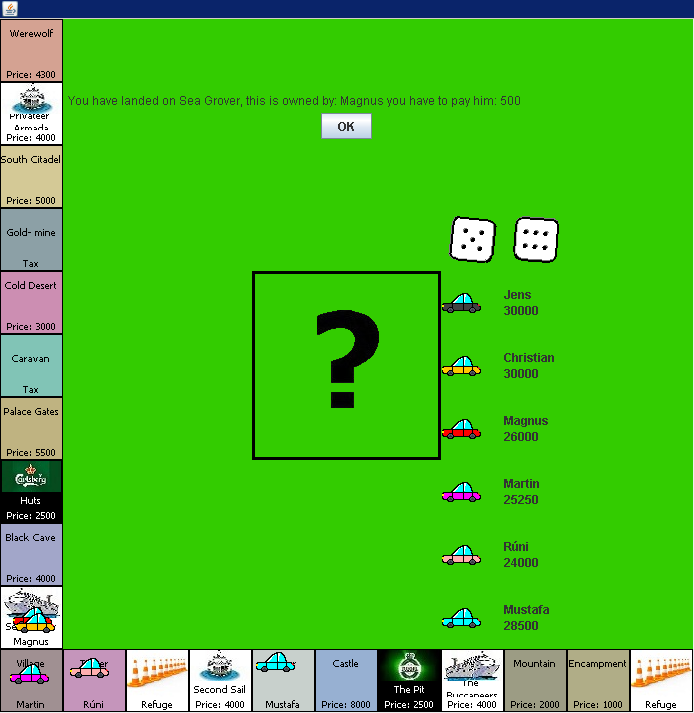
\includegraphics[width=0.8\paperwidth]{bilag02}}
\caption{\emph{Bilag 2}: Spilleren betaler leje.}
\end{figure}
\FloatBarrier
\begin{figure}[h]
\section*{Bilag 3}\label{bilag3}
\centering
\makebox[\textwidth]{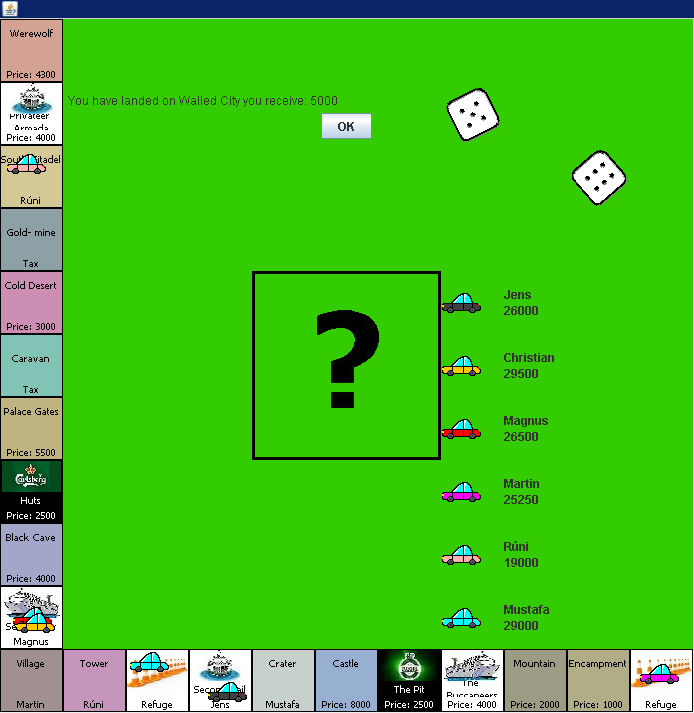
\includegraphics[width=0.8\paperwidth]{bilag03}}
\caption{\emph{Bilag 3}: Spilleren modtager penge på ‘Refuge’.}
\end{figure}
\FloatBarrier
\begin{figure}[h]
\section*{Bilag 4}\label{bilag4}
\centering
\makebox[\textwidth]{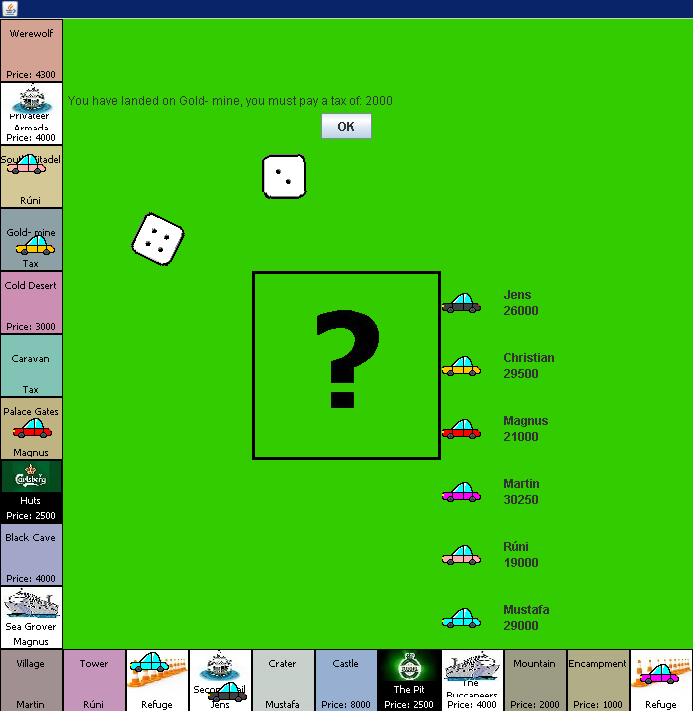
\includegraphics[width=0.8\paperwidth]{bilag04}}
\caption{\emph{Bilag 4}: Spilleren betaler fast skat på ‘Tax’.}
\end{figure}
\FloatBarrier
\begin{figure}[h]
\section*{Bilag 5}\label{bilag5}
\centering
\makebox[\textwidth]{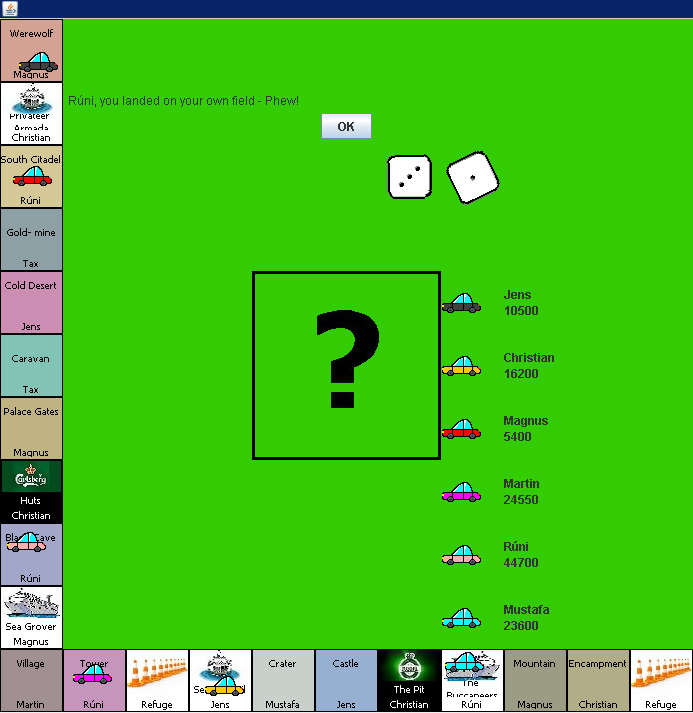
\includegraphics[width=0.8\paperwidth]{bilag05}}
\caption{\emph{Bilag 5}: Spilleren lander på eget felt.}
\end{figure}
\FloatBarrier
\begin{figure}[h]
\section*{Bilag 6}\label{bilag6}
\centering
\makebox[\textwidth]{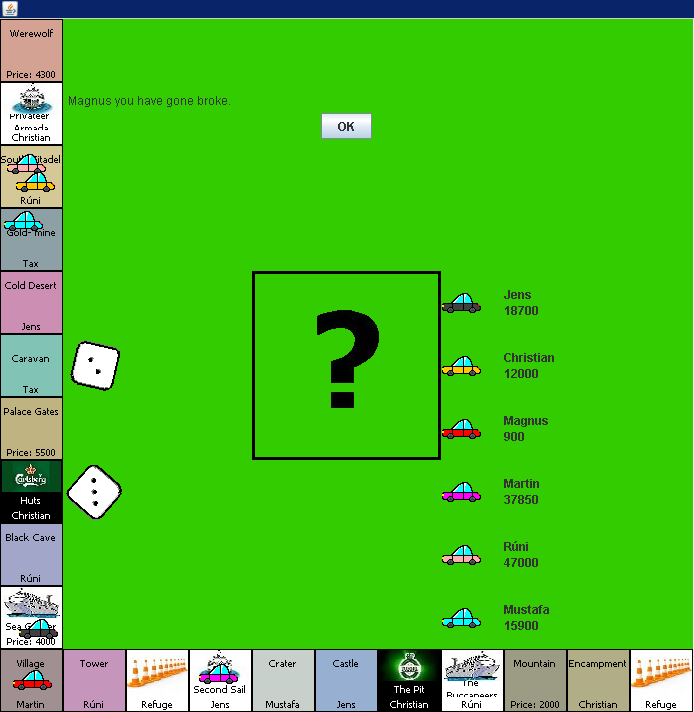
\includegraphics[width=0.8\paperwidth]{bilag06}}
\caption{\emph{Bilag 6}: Spilleren går fallit.}
\end{figure}
\FloatBarrier
\begin{figure}[h]
\section*{Bilag 7}\label{bilag7}
\centering
\makebox[\textwidth]{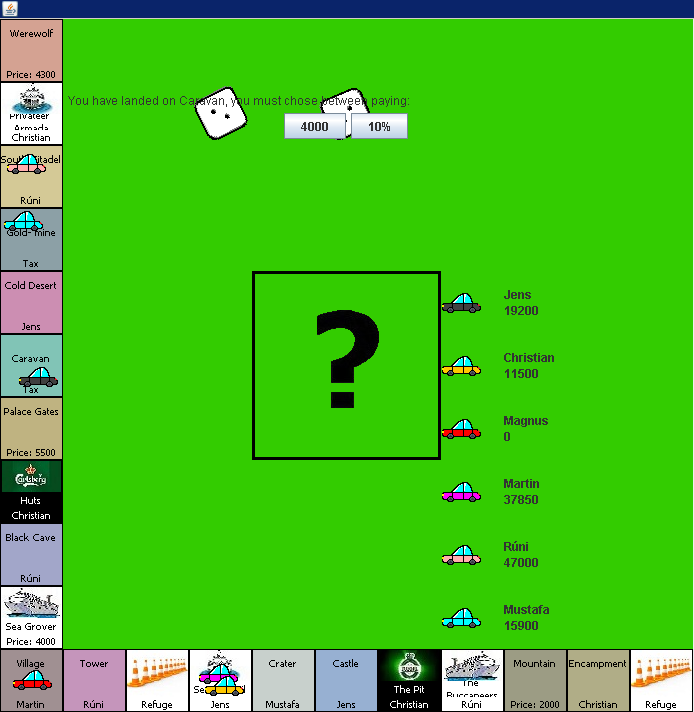
\includegraphics[width=0.8\paperwidth]{bilag07}}
\caption{\emph{Bilag 7}: Spilleren lander på et variabelt ‘Tax’ felt.}
\end{figure}
\FloatBarrier
\begin{figure}[h]
\section*{Bilag 8}\label{bilag8}
\centering
\makebox[\textwidth]{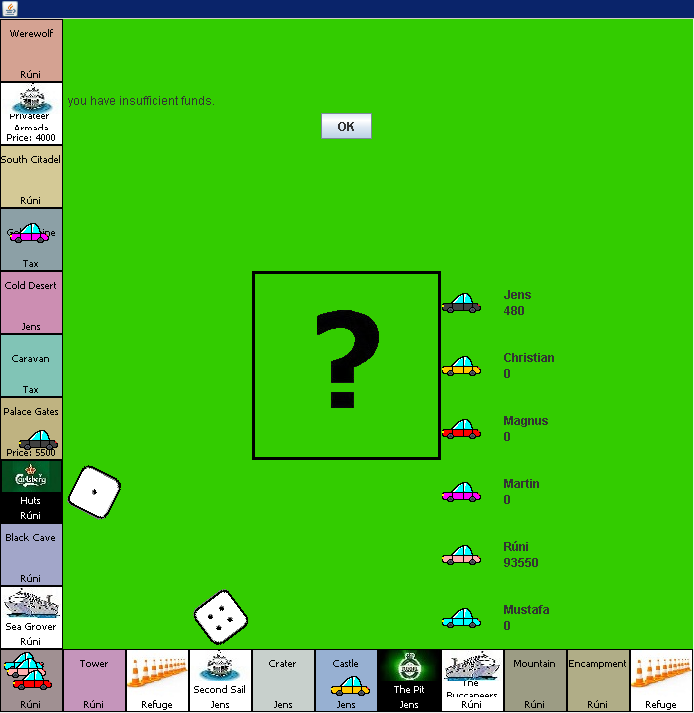
\includegraphics[width=0.8\paperwidth]{bilag08}}
\caption{\emph{Bilag 8}: Spilleren har ikke råd til at købe feltet.}
\end{figure}
\FloatBarrier
\begin{figure}[h]
\section*{Bilag 9}\label{bilag9}
\centering
\makebox[\textwidth]{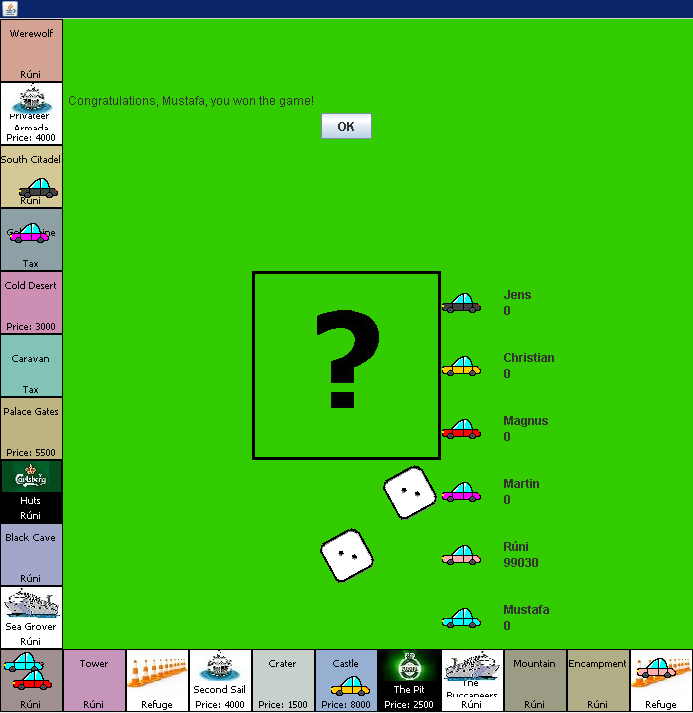
\includegraphics[width=0.8\paperwidth]{bilag09}}
\caption{\emph{Bilag 9}: Fejlagtig udnævnelse af vinderen - rettet i senere udgave.}
\end{figure}
\FloatBarrier
\begin{figure}[h]
\section*{Bilag 10}\label{bilag10}
\centering
\makebox[\textwidth]{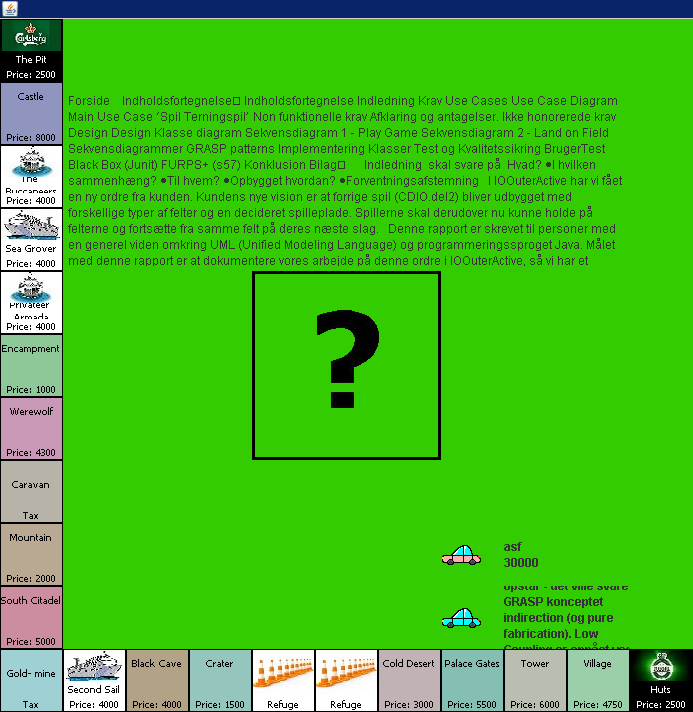
\includegraphics[width=0.8\paperwidth]{bilag10}}
\caption{\emph{Bilag 10}: Spilleren har valgt et meget langt navn - Hvilket får
ok knappen til at ‘forsvinde’ og gør spillet uspilleligt.}
\end{figure}
\FloatBarrier
\begin{figure}[h]
\section*{Bilag 11}\label{bilag11}
\centering
\makebox[\textwidth]{\includegraphics[width=0.8\paperwidth]{bilag11}}
\caption{\emph{Bilag 11}: Spillerne har valgt ens navne - Hvilket GUI’en ikke
kan håndtere.}
\end{figure}
\FloatBarrier
\end{appendices}